%%%% I-POMCP: supplementary material for the IJCAI-27 submission

\documentclass{article}
\usepackage[margin=1in]{geometry}
\usepackage{times}
\usepackage[utf8]{inputenc}
\usepackage{amsmath}
\usepackage{amssymb}
\usepackage{booktabs}
\usepackage{algorithm}
\usepackage{algorithmic}
\usepackage{tikz}
\usetikzlibrary{arrows.meta,positioning,fit,calc}

% Notation of the main paper
\newcommand{\IS}{\mathit{IS}}
\newcommand{\SE}{\mathit{SE}}
\newcommand{\ER}{\mathit{ER}}
\newcommand{\OPT}{\mathit{OPT}}
\newcommand{\SEN}{\widetilde{\SE}^{N}}
\newcommand{\hth}{\hat{\theta}}
\renewcommand{\Pr}{\mathit{Pr}}

\title{Interactive POMCP: Supplementary Material}
\author{Anonymous Submission}
\date{}

\begin{document}
\maketitle

\section{Overview and Pseudocode}

Figure~\ref{fig:overview} summarizes the search, and Algorithm~\ref{alg:filter} gives the compressed update of Section~4.1 of the paper together with the recursive solution of the other agent's models (Section~4.4).

\begin{figure}[h]
\centering
\resizebox{0.8\textwidth}{!}{%
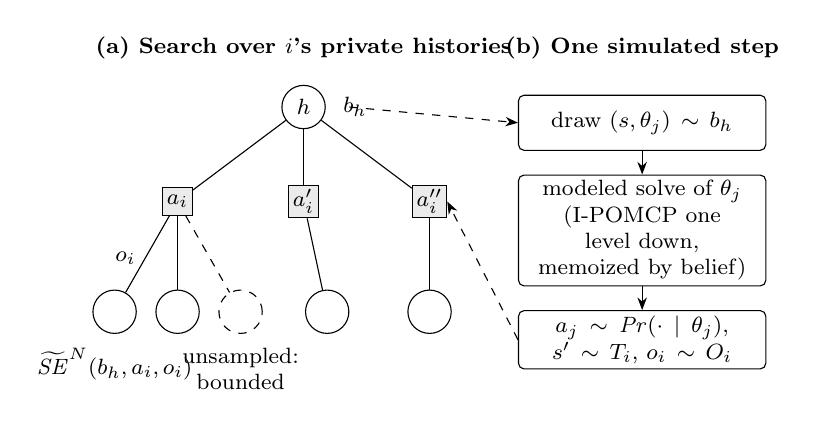
\begin{tikzpicture}[
    font=\footnotesize,
    box/.style={draw, rounded corners=2pt, align=center, inner sep=2pt, minimum height=0.7cm},
    hist/.style={draw, circle, inner sep=1.2pt, minimum size=0.55cm},
    act/.style={draw, fill=black!8, rectangle, inner sep=1.5pt, minimum size=0.35cm},
    arr/.style={-{Stealth[length=1.6mm]}},
    dasharr/.style={-{Stealth[length=1.6mm]}, dashed}
]
% (a) search tree
\node[hist] (h) at (0,0) {$h$};
\node[right=0.1cm of h, align=left] {$b_h$};
\node[act] (a1) at (-1.6,-1.2) {$a_i$};
\node[act] (a2) at (0,-1.2) {$a_i'$};
\node[act] (a3) at (1.6,-1.2) {$a_i''$};
\draw (h) -- (a1); \draw (h) -- (a2); \draw (h) -- (a3);
\node[hist] (c1) at (-2.4,-2.6) {};
\node[hist] (c2) at (-1.6,-2.6) {};
\node[hist, dashed] (c3) at (-0.8,-2.6) {};
\draw (a1) -- node[left, pos=0.55] {$o_i$} (c1);
\draw (a1) -- (c2);
\draw[dashed] (a1) -- (c3);
\node[below=0.05cm of c1, align=center] {$\SEN(b_h, a_i, o_i)$};
\node[below=0.05cm of c3, align=center, text width=1.6cm] {unsampled:\\ bounded};
\node[hist] (c4) at (0.3,-2.6) {};
\draw (a2) -- (c4);
\node[hist] (c5) at (1.6,-2.6) {};
\draw (a3) -- (c5);
\node[font=\footnotesize\bfseries] at (0,0.75) {(a) Search over $i$'s private histories};

% (b) modeled solve
\node[box, text width=3.0cm] (draw) at (4.3,-0.2) {draw $(s, \theta_j) \sim b_h$};
\node[box, text width=3.0cm, below=0.3cm of draw] (solve) {modeled solve of $\theta_j$\\ (I-POMCP one level down,\\ memoized by belief)};
\node[box, text width=3.0cm, below=0.3cm of solve] (step) {$a_j \sim \Pr(\cdot \mid \theta_j)$,\\ $s' \sim T_i$, $o_i \sim O_i$};
\draw[arr] (draw) -- (solve);
\draw[arr] (solve) -- (step);
\draw[dasharr] (h.east) ++(0.3,0) -- (draw.west);
\draw[dasharr] (step.west) -- (a3.east);
\node[font=\footnotesize\bfseries] at (4.3,0.75) {(b) One simulated step};
\end{tikzpicture}}
\caption{Overview of I-POMCP. (a) The search tree over $i$'s own histories; every history $h$ carries $i$'s interactive belief $b_h$, computed with the compressed filter $\SEN$, and observation branches that search did not sample enter the certified intervals at the bounds of the reward range. (b) In a simulated step, an interactive state is drawn from $b_h$, and the other agent acts by the solution of its own model.}
\label{fig:overview}
\end{figure}

\begin{algorithm}[h]
\caption{Compressed update and modeled solves}
\label{alg:filter}
\begin{algorithmic}[1]
\STATE \textbf{procedure} \textsc{Policy}$(\theta_j)$ \hfill ($\theta_j$ at level $k$)
\IF{$k = 0$}
    \STATE \textbf{return} the uniform distribution over $A_j$
\ENDIF
\IF{the canonical digest of $\theta_j$ is cached}
    \STATE \textbf{return} the cached policy
\ENDIF
\STATE run Algorithm~1 of the paper for $j$ at $b_j$ with the modeled budget, solving $j$'s models of $i$ by \textsc{Policy} at level $k-1$
\STATE \textbf{return} the uniform distribution over $\arg\max_{a_j} Q^\star$, and cache it
\STATE
\STATE \textbf{procedure} $\SEN_{\theta_i}(b_i, a_i, o_i)$
\STATE $b' \leftarrow 0$
\FORALL{$(s, \theta_j) \in \mathrm{supp}(b_i)$, $a_j$ with $\pi = \textsc{Policy}(\theta_j)(a_j) > 0$, $s'$, $o_j$}
    \STATE $w \leftarrow b_i(s, \theta_j)\, \pi\, T_i(s, a, s')\, O_i(s', a, o_i)\, O_j(s', a, o_j)$
    \STATE $\theta_j' \leftarrow \langle \SEN_{\theta_j}(b_j, a_j, o_j), \hth_j \rangle$ \hfill (unchanged at level 0)
    \STATE $b'(s', \theta_j') \leftarrow b'(s', \theta_j') + w$ \hfill (canonical merge)
\ENDFOR
\STATE normalize $b'$
\IF{$|\mathrm{supp}(b')| > N$}
    \STATE $b' \leftarrow$ $N$ stratified draws from $b'$ in canonical order, merged
\ENDIF
\STATE \textbf{return} $b'$
\end{algorithmic}
\end{algorithm}


\paragraph{Adaptive modeled budget.} A modeled solve grows one search tree by doubling its number of simulations from a small pilot size. After each doubling it compares the gap between its two leading actions with a Bonferroni-corrected $t$ critical value times the spread of the same gap across a few independent pilot trees, and it stops as soon as the gap exceeds that threshold. At its cap, the solve is identical to a flat search with the cap's budget, so the rule is consistent.

\section{Domains}

\begin{table}[h]
\centering
\begin{tabular}{@{}lrrrl@{}}
\toprule
Domain & $|S|$ & $|A_i|$ & $|A_j|$ & Observations \\
\midrule
Tiger (both games) & 2 & 3 & 3 & 6 per agent \\
UAV reconnaissance & 81 & 5 & 5 & 3 / 27 \\
Wumpus world, $3 \times 3$ & 2{,}048 & 5 & 3 & percept sets \\
\bottomrule
\end{tabular}
\caption{The domains. For the Wumpus world, $|S|$ counts the initial states.}
\label{tab:domains}
\end{table}

\paragraph{Multi-agent tiger.} Two agents face two doors, one hiding a tiger and the other a prize. Each agent can listen or open a door; listening costs 1, opening the tiger's door costs 100 and opening the other door pays 10, and if either agent opens a door the tiger is placed at random. A listening agent hears the tiger's growl from the correct side with probability 0.85, together with a creak that reports the other agent's action with probability 0.9. In the \emph{coordination} game, an agent that opens the safe door in the same step as the other agent receives 40 instead of 10.

\paragraph{UAV reconnaissance.} An unmanned aerial vehicle $i$ seeks a ground target $j$ on a $3 \times 3$ grid of sectors. Both agents move to an adjacent sector or stay. The UAV knows its own sector and, when it stays, observes the target's row with probability 0.8; the target knows its own sector and observes the UAV's row with probability 0.6. The UAV receives 50 for spotting the target, which ends the episode, and pays 5 for every other step; the target loses 50 when spotted. Parameters that the original description leaves open follow Zeng and Doshi (2012).

\paragraph{Two-agent Wumpus world.} A human $i$ searches a $3 \times 3$ grid with one pit for gold, while a wumpus $j$ hunts the human. The human can move forward, turn, grab and shoot one arrow; the wumpus can move forward and turn. Both agents perceive deterministic sets of tokens: the human perceives bump, stench, breeze, glitter and scream, and the wumpus perceives bump, breeze, glitter and the human's footsteps within distance 2. The human receives 1000 for the gold and $-1000$ for dying, and the wumpus 1000 for catching the human and $-1000$ for being shot; every other step costs 1.

\section{The Released Variant of I-NTMCP}

The released code of I-NTMCP refills a belief after a real step by rejection sampling and, after 3{,}000 rejections, fills the rest with particles whose own observation contradicts the real one. Under the Wumpus world's deterministic percepts this \emph{force-filling} grows with the budget: in the 60 level-2, horizon-2 problems of Table~1 of the paper, the median force-filled share is 0, 0.17 and 0.43 at $M = 1{,}000$, 4{,}000 and 16{,}000 (maximum 0.99), and the released variant is optimal on 19, 32 and 29 of 60 problems, against 17, 32 and 34 for the reinvigorated variant. In the 20-step UAV episodes at horizon 4, the released variant force-fills 31--49\% of its beliefs on average at $M \geq 4{,}000$; it earns 17.5, 20.8, 32.2 and 35.0 at $M = 1{,}000$ to 64{,}000 ($n = 30$), and is optimal on 73--88\% of the exactly scored decisions for $M \leq 16{,}000$, against 120 of 120 for I-POMCP at budget 1{,}000.

\section{Fidelity of the Baselines}

\paragraph{I-NTMCP.} On the authors' own Runner-Chaser $4 \times 4$ problem (Schwartz et al., 2022), their runner, unchanged, reproduces their published results exactly: the runner earns 65.964 (standard deviation 71.2) against a random chaser and 95.998 against a level-0 chaser, over 1{,}000 episodes each. We restated the problem as finite transition, observation and reward functions, which agree with the authors' model on every state and joint action, and ran the same planner (nesting level 1, 1{,}024 simulations, the published exploration constant) through our adapter: it earns 65.57 (71.6) against the random chaser, a difference of $-0.40$ within the two-sample 95\% half-width of 6.26, and reaches safety in 847 of 1{,}000 episodes against the authors' 849. A search through the adapter costs 1.45 times the CPU of the authors' runner, so the CPU comparisons of the paper charge I-NTMCP up to that factor.

\paragraph{IPF + RTS.} We rebuilt the multiagent tiger setting of Doshi and Gmytrasiewicz (2009, Fig.~17(a): horizon 3, $N_p \in \{50, 100\}$ particles, $K$ sampled observations per node; agent $i$ uninformed about the tiger and about $j$'s belief; 10 policy trees and 100 runs per point). Used as in our experiments, replanning at every reached history, our implementation earns $-0.5$ to $+0.8$ at every $K$ from 2 to 10, the level the published curve reaches at $K \geq 10$. The published losses at small $K$ ($-20.5$ to $-14.6$ at $K \leq 3$) arise from executing one policy tree built from $K$ sampled observations: in 72--74\% of runs at $K = 2$ the real observation is missing from the tree. Executing such a tree, with listening or a uniformly random action once the tree is left, brackets the published value at all 12 points.

\section{Decisions at Chosen Beliefs}

I-POMCP's budgets were chosen on grids of named beliefs: for the tiger games, $i$'s belief about the tiger crossed with $j$'s and, from level 3, with the beliefs below $j$; for UAV reconnaissance, named distributions over the other agent's sector; for the Wumpus world, beliefs reachable from the common prior. Table~\ref{tab:decisions-supp} gives the decisions on these grids. The configurations were then rerun, unchanged, on 960 random tiger beliefs and seeds that no selection used (levels 2 and 3, both games): all 960 decisions are optimal. In the original tiger game at level 3 and horizon 4, 76 of 80 decisions are optimal and the other four lose at most 0.03. At level 3 and horizon 3, exact scoring with two steps to go reduces the error of the optimal action's value from 0.06 to 0.0006.

\begin{table}[h]
\centering
\footnotesize
\setlength{\tabcolsep}{3pt}
\begin{tabular}{@{}llrrrrr@{}}
\toprule
Domain & $l$, $H$ & $n$ & I-POMCP & IPF + RTS & I-NTMCP & Exact CPU (s) \\
\midrule
Tiger (orig.) & 1, 5 & 220 & 220 & -- & -- & 0.009 \\
 & 2, 3 & 380 & 380 & 374--378 & -- & 0.05 \\
 & 2, 4 & 380 & 380 & 362--368 & -- & 1.0 \\
 & 3, 3 & 162 & 162 & -- & -- & 6.3 \\
Tiger (coord.) & 3, 2 & 162 & 162 & 148--158 & -- & 0.006 \\
 & 3, 3 & 162 & 162 & 150--159 & -- & 0.34 \\
 & 4, 2 & 486 & 486 & -- & -- & 0.05 \\
UAV & 1, 2--5 & 40 each & 40 each & -- & -- & 0.01--1.3 \\
 & 2, 2 & 80 & 80 & 46--55 & -- & 0.17 \\
 & 2, 3 & 80 & 80 & 42--48 & -- & 2.0 \\
 & 2, 4 & 80 & 80 & 37--40 & -- & 24 \\
 & 3, 2 & 320 & 320 & -- & -- & 0.25 \\
Wumpus & 2, 2 & 60 & 60 & 1--26 & 40 & 75 \\
 & 3, 2 & 55 & 55 & -- & -- & 74 \\
\bottomrule
\end{tabular}
\caption{Optimal decisions against the exact I-POMDP at level $l$ and horizon $H$, out of $n$ problems. IPF + RTS: the range over $K \in \{2, 4, 8\}$ and, where both were run, over the plain and smoothed filters. I-NTMCP: $M = 64{,}000$, at 0.8 times I-POMCP's CPU. Exact CPU: the exact I-POMDP solver's median CPU per decision on the same grid (one problem per process; 9 problems per row drawn at random, all 4 at UAV level 1, all $n$ for the Wumpus world). On the tiger and UAV grids, which hold beliefs at the start of play, the exact solver is cheap; Section~7.1 compares the two at beliefs reached by play.}
\label{tab:decisions-supp}
\end{table}

\section{Anytime UAV Episodes}

A level-2 UAV plans with $H = 4$ or 5 in 20-step episodes from the common prior against a level-1 I-POMCP target ($n = 30$ per planner and budget). The exact solver cannot play such episodes, since its cost per decision grows about threefold with each step of history, but it can score their first decisions. I-POMCP uses root budgets of 50 to 1{,}000 simulations and models the target with the same budget, and I-NTMCP uses $M$ from 1{,}000 to 64{,}000. The decisions at the first five steps of each $H = 4$ episode are scored exactly; the exact solver's median CPU on them grows from 10~s at the first step to 710~s at the fifth. I-POMCP at $H = 4$ earns 34.8 at 2.9 s per decision (35 is the most any episode earned), where I-NTMCP earns 20.8 at 3.7 s and 32.2 at 13 s. With no more CPU than I-NTMCP, I-POMCP earns 2.7 [1.7, 3.7] more than I-NTMCP at $M = 16{,}000$ and 2.5 [1.2, 4.0] more at $M = 16{,}000$ and $H = 5$ (Holm $p \leq 0.01$), and 14.0 [4.3, 27.5] more at $M = 4{,}000$ (Holm $p = 0.12$); at $M = 64{,}000$, 55 s per decision, both always spot the target after four steps. Over the first five decisions at $H = 4$, I-POMCP at budget 1{,}000 is optimal on 120 of 120 at a median of 15~s per decision, against 51~s for the exact solver on the same decisions, I-NTMCP on 73--88\% for $M \leq 16{,}000$, and IPF + RTS ($K = 2$, over 1{,}100 s per decision) on 62--70\%. These episodes were run before the tie rule of the main text (exact values within a relative $10^{-9}$ are tied); the comparison is paired on the same target, and I-NTMCP is reported in its stronger variant at each $M$.

\section{Reproducibility}

\paragraph{Computing infrastructure.} All experiments ran on one machine with an Intel Core Ultra 9 275HX (24 cores) and 23~GB of memory under Linux (WSL2), with Python 3.12. Every planner is single-threaded and runs one decision or episode per process; we report the process CPU time of a decision, nested solves included, so that times do not depend on how many processes share the machine.

\paragraph{How budgets were chosen.} For I-POMCP, the root budget was tried over $\{100, 250, 1{,}000, 4{,}000, 16{,}000, 64{,}000\}$ simulations, the modeled budget over $\{100, 400, 1{,}600, 6{,}400\}$ and sequential stopping capped at 6{,}400, and the belief bound over $N \in \{32, 64, 256, 1{,}024\}$ and exact beliefs. On each grid of named beliefs (Table~\ref{tab:decisions-supp}) we chose the smallest budget at which every decision was optimal against the exact I-POMDP, and then tested it, unchanged, on beliefs and seeds that the selection did not use (960 random tiger beliefs; 219 reachable Wumpus beliefs). The near-tie escalation threshold $g = 3$ was fixed before its held-out test. No parameter of a baseline was tuned on our problems: IPF + RTS and I-NTMCP were run over ladders of their own budgets, and every arm is reported.

\paragraph{Final settings.} Unless stated, $\gamma = 0.95$ and the exploration constant is $c = 1$. Sequential stopping uses 200-simulation pilots, 4 trees and $\alpha = 0.01$.
\begin{itemize}
\item Tiger decisions: level 2, horizon 3, root 1{,}000, modeled 400, exact beliefs; level 3, horizon 3, root 1{,}000, modeled stopping capped at 6{,}400 for level 2 and 100 for level 1; horizon 2, root 100, modeled 100, $N = 32$.
\item Tiger level grid: horizon 2, 100 simulations at the root and in every modeled solve, $N = 64$. Near-tie escalation (separate episodes, Section~7.2): $N' = 1{,}024$ at level 2 and 256 at levels 3--4, $g = 3$.
\item UAV decisions: horizons 2--3, root 1{,}000, target 100 (horizon 2) or 400 (horizon 3), $N = 64$; horizon 4, root 16{,}000 with an exact or 6{,}400-simulation stopped target; level 1 at horizon 5, root 64{,}000. At reachable beliefs (Section~7.1), root 1{,}000, target 1{,}600, exact beliefs.
\item UAV level matrix: horizon 3, root 1{,}000, $N = 64$, the same budget for every modeled level.
\item Wumpus world: horizon 2, exact beliefs, root and modeled 400 (episodes and reachable beliefs) or root 1{,}000 and modeled 400 (decision grids).
\item IPF + RTS: $N = 64$ particles at every level, $K \in \{2, 4, 8\}$ sampled observations per node, smoothing $\epsilon = 0.01$ where stated.
\item I-NTMCP: the authors' defaults (exploration constant $R_{\max} - R_{\min}$, uniformly random rollouts, $1/16$ extra particles per step), $M \in \{1{,}000, 4{,}000, 16{,}000, 64{,}000\}$, discount horizon set so that the search depth equals $H - 1$; the reinvigorated variant allows 50 rejections per particle.
\end{itemize}

\paragraph{Code.} The code archive submitted with this supplement contains the planner, the exact references, the baselines' adapters, the domains, the test suite and the scripts of every experiment in the paper; it will be released under the MIT license upon publication. I-NTMCP is the authors' public implementation, used unchanged.

\section{Ablations}

\begin{table}[h]
\centering
\small
\begin{tabular}{@{}p{0.3\textwidth}p{0.64\textwidth}@{}}
\toprule
Component & Paired evidence \\
\midrule
Exact scoring at the root & Turning it off makes 34 of 560 UAV decisions suboptimal and none optimal (exact McNemar $p = 1.2 \times 10^{-10}$); it changes none of 1{,}786 tiger decisions \\
Exact scoring with two steps left & Error of the optimal action's value at level 3, horizon 3: 0.06 without, 0.0006 with \\
Compressed exact filter instead of the particle filter & Wumpus world: the particle filter fails on 55--57 of 60 problems; RTS on exact beliefs matches the smoothed particle filter \\
Stratified instead of systematic compression & Systematic draws alias a pit cell on uniform beliefs (12 of 60 problems lose 102.5); stratified draws fix 31 of 34 discordant pairs and are worse on none \\
Adaptive modeled budget & Same decisions as a flat 6{,}400 simulations at 0.52 times its CPU \\
Root budget 1{,}000 instead of 4{,}000 & Error of the optimal action's value at level 2, horizon 4: 0.121 against 0.031, at 1.06 times the CPU \\
Level priors with level-0 mass & A wrong point prior over the other agent's level costs 17.5--30.0 per episode, a uniform prior nothing significant; level-0 mass keeps the Wumpus updates at level 3 defined \\
\bottomrule
\end{tabular}
\caption{What each component buys, from paired comparisons on the same problems or episodes.}
\label{tab:ablations}
\end{table}

\end{document}
